
 % -*- coding: utf-8 -*-
%\documentclass[english]{ipsj}
%\documentclass[english,preprint]{ipsj}
\documentclass[english,preprint,JIP]{ipsj}

\usepackage{graphicx}
\usepackage{latexsym}

\def\Underline{\setbox0\hbox\bgroup\let\\\endUnderline}
\def\endUnderline{\vphantom{y}\egroup\smash{\underline{\box0}}\\}
\def\|{\verb|}


\setcounter{volume}{26}% vol25=2017
\setcounter{number}{1}%
\setcounter{page}{1}


\received{2016}{3}{4}
%\rereceived{2011}{10}{1}   % optional
%\rerereceived{2011}{10}{31} % optional
\accepted{2016}{8}{1}



\usepackage[varg]{txfonts}%%!!
\usepackage{url}

\makeatletter%
\input{ot1txtt.fd}
\makeatother%

\begin{document}

\title{Magnet or Sticky? A Stack Overflow Tag-by-Tag Typology\\}

% \affiliate{IPSJ}{Information Processing Society of Japan, 
% Chiyoda, Tokyo 101--0062, Japan}
% \affiliate{JU}{Johoshori University, Chiyoda, Tokyo 101--0062, Japan}
% \paffiliate{PJU}{Johoshori University}

\author{Kotori Hieda}{IPSJ,PJU}
\author{Yu Mingzhe}{JU}
\author{Yasutaka Kamei}{IPSJ}


\begin{abstract}
Stack Overflow (SO) is one of the most popular question and answer websites among software developers. SO stores posts with tags that indicate the keyword that categories the question. For example, if a developer asks about Python and puts ``Python'' tag on the post, the developers who are interested in Python can easily find and answer the post. SO has started its service since 2008 and is still becoming popular. Therefore, we explore how developers' interest shift by analyzing how they use tags. We classify tags into four types: (1) attractive, (2) stagnant, (3) fluctuating, and (4) terminal based on magnet values and sticky values. We analyze the data from table ``Posts'' which includes about 42 million posts from Stack overflow and table ``Users'' where there are about 9 million rows of user information. Results reveal that: 
(1) There were some historical events in IT such as the launch of new tools and the termination of services when there were characteristics in the transition of magnet value and sticky value.
(2) The types of tags that are classified do not change much.
\end{abstract}

\begin{keyword}
magnet, sticky, tag, user migration, OSS census
\end{keyword}

\maketitle

%1
\section{Introduction}
Pew Research Center~\cite{communityeconomic}, an organization that studies problems in the United States and the world, investigated society and population using US tax survey data.  States that have a high percentage of people migrating from the outside are defined as \emph{magnet states} and states where the high proportion of the population who continues to live in the same state since birth are defined as \emph{sticky states}. For example, 86\% of Nevada's population migrated from other states so Nevada state is quite \emph{magnet}. Through such a survey, we can find the tendency how American citizens move.

For software developers, it is important to know the changes in the interests of other developers because popularity among many developers should have advantages. Developers always want to work with convenient and easy-to-use tools. To make a project better, excellent developers need to be interested in the project over the long term.

Therefore, in this study, we focus on new and existing interests in the topics of StackOverflow. Inspired by previous studies~\cite{yamashita2016magnet}, we apply Magnet and Sticky metrics to the topics that are collected in StackOverflow. 
The Magnet metric indicates the number of new developers attracted to a topic and Sticky metric indicates the number of existing developers that stay with the topic. 
We examined tags' magnets and sticky values by classifying them as the tags \emph{programming language}, \emph{framework}, and \emph{environment}. We also compared the news and history of software companies and web services, if there are characteristic changes in magnet values and sticky values, we examined why it was like that. We addressed the following two research questions:

\noindent \textbf{(RQ1) What are typical values of magnet and sticky in Stack Overflow?}\par
In many cases, the sticky value tended to be higher than the magnet value. In addition, the decrease rate was higher for the magnet value than for the sticky value. If it is easy to use and convenient like the .NET Framework, the magnet value and the sticky value are high.

\noindent \textbf{(RQ2) How do magnet and sticky values change over time?}\par
We can identify which tags are obsolete. When the tags move quadrant, we find that something happens.


\section{Definition of Magnet and Sticky} \label{magnet}
This section describes how we measure the appeal and adhesion of users on different topics on Stack Overflow in this study, we use the Magnet and Sticky metrics defined by the Pew Research Center for illustrating the migratory trends of citizens in the United States.

The Pew Research Center report defines magnet states as those states where a large proportion of adults who live there have moved from another state. Thus, the magnet metric for a state is the proportion of adult residents of a state who were not born in the state. Furthermore, the report also defines sticky states as those states where a large proportion of adults who were born there continue to live there. Thus, the sticky metric for a state is the proportion of adult residents who were born in the state

These definitions are sound for a study of populations, where a single adult can only occupy one state at a time. However, the definition cannot be applied directly to the topics discussed by the users of Stack Overflow where a user can ask or answer questions on several topics at the same time. Therefore, we expand new definition to apply to topics in Stack Overflow as follows:

\subsection*{\textit{\textbf{Magnet and Sticky in Stack Overflow}}}

Questions in Stack Overflow are composed of the content of the question, answers to the questions and comments~\cite{liu2018mining}, that are call Posts in the database of SOTorrent. Each question has one or more tags that separate the question into different topics. Simultaneously, posts in a question have their own creator (for the question content, one is the questioner, and for the answer, one is the respondent) who is a participant of the topics of the question. We also define the activity of asking or answering questions on some topic as a discussion of the topic. For example, a classical question in Stack overflow has three tags like java, apache, and Linux which is asked by user A and answered by user B, and C, so A, and C are participants of topic java, apache, and Linux.

\noindent
\textbf{Magnet.} Magnet topics are those that attract a large proportion of new users. Thus, we calculate the magnetism of a topic as the proportion of users who ask or answer during the time period under research to all new users who registered their account at the year.

\noindent
\textbf{Sticky.} Sticky topics are those where a large proportion of the users will keep participating in the discussion in the time period under research and the following. Thus, we calculate the stickiness of a topic as the proportion of the users who discuss within the topic in the time period under research to who have also discussed in the following time period.

\noindent
\textbf{Example (Calculating magnet and sticky values).}
Let us explain how we calculate magnet and sticky values for some topics belong to a major category as an example. There are 6 questions (a, b, c, d, e, f) and 7 users (A, B, C, D, E, F, G), the Last Activity Date of question a, b, c is during 2017 and question d, e, f is during 2018. The registration date of user A, B, C, D is during 2017 and the registration date of user E, F, G is during 2018~\cite{yamashita2016magnet}.

\begin{figure}[t]
 \centering
 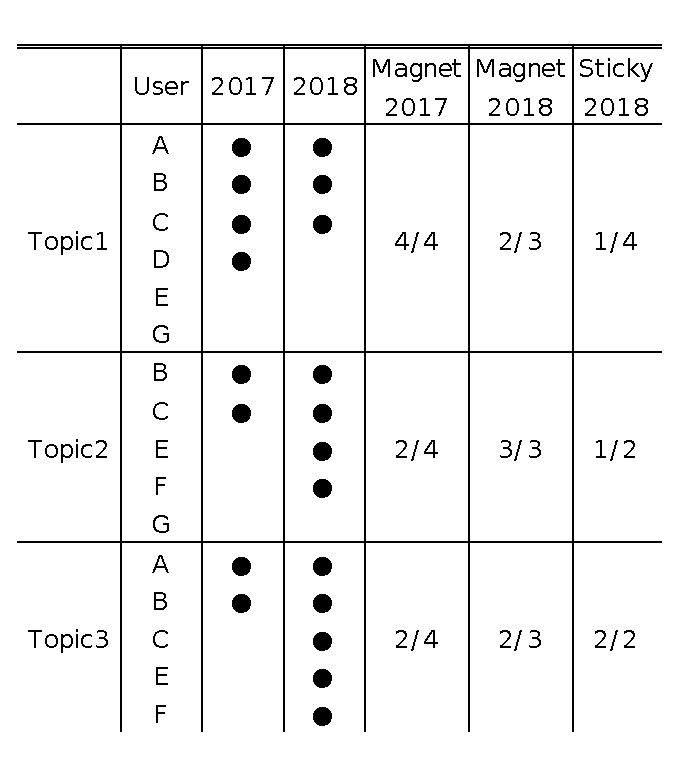
\includegraphics[width=.75\hsize]{img/explainofMS.eps}  
 \caption{Example of Magnet and Sticky values definition} 
 \label{fig:example2} 
\end{figure}


To calculate the magnet metric, we observe that there are four new users who register his/her account in 2017 (A, B, C, and D), and all of them discuss in topic 1, while two of them (B, C) participate in the discussion of topic 2 and 3. In this case, Magnet value of topic 1 in 2017 is 4/4, topic 2 is 2/4 and topic 3 is 2/4.

To calculate the sticky metric, on topic 1, there are three users participate in the discussion in 2017 (A, B and C) but only one of them also participate in the discussion in 2018 (A). Hence, the sticky value of project 1 is 1/4. on topic 2, there are 2 users participate in the discussion in 2017 (B and C) but only one of them also participate in the discussion in 2018 (B). Even though new users E F G participate in the discussion in 2018, we still calculate the value of sticky as 1/2. For the same reason, the sticky of topic 3 is 2/2 in 2018.\\

\noindent
\textbf{Example (Merging similar subjects into one topic).}
We merge subjects (i.e., tags) belonging to analogous subjects into one topic. For example, we consider that different version number suffixes (e.g., ``python-2.7'' and tag ``python-3.6'') are one of the common examples of analogous tags. 

\begin{figure}[t]
 \centering
 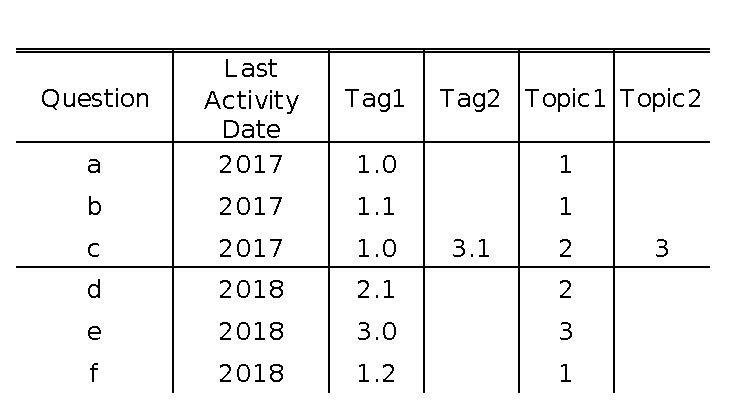
\includegraphics[width=0.80\hsize]{img/example001.eps}  
 \caption{Example of the merge of tags belonging to analogous subjects} 
 \label{fig:example1} 
\end{figure}


We also consider that we need merge include derivatives of the same technology on different platforms, special tools in a certain tool family, or a combination of a technology with its commonly used library, etc. For example, tag ``reactjs'', ``react-router'', ``reactjs-flux'', ``create-react-app'' should be merged into one topic ``react''.
% Of course, the difference in version number is the most common example of analogous tags. The rest of examples includes derivatives of the technology on different platforms, commonly used libraries, or specific tools in a tool family, etc. for example topic ``react'' includes tag ``reactjs'', ``react-router'', ``reactjs-flux'', ``create-react-app'' etc. 
We can get this information from the ``Related Tag'' column of the ``Tag Info'' on Stack Overflow.''

Figure~\ref{fig:example1} shows that question a has tag 1.0, question b has tag 1.1 and question f has tag 1.2 , which means according to our merge rule, they all belong to topic 1.  Simultaneously, question c has tag 2.0 and tag 3.1, which means it belongs to topic 2 and 3 at the same time. Therefore, queston d belongs to topic 2 and question e belongs to topic 3.


\begin{figure*}[t]
 \centering
 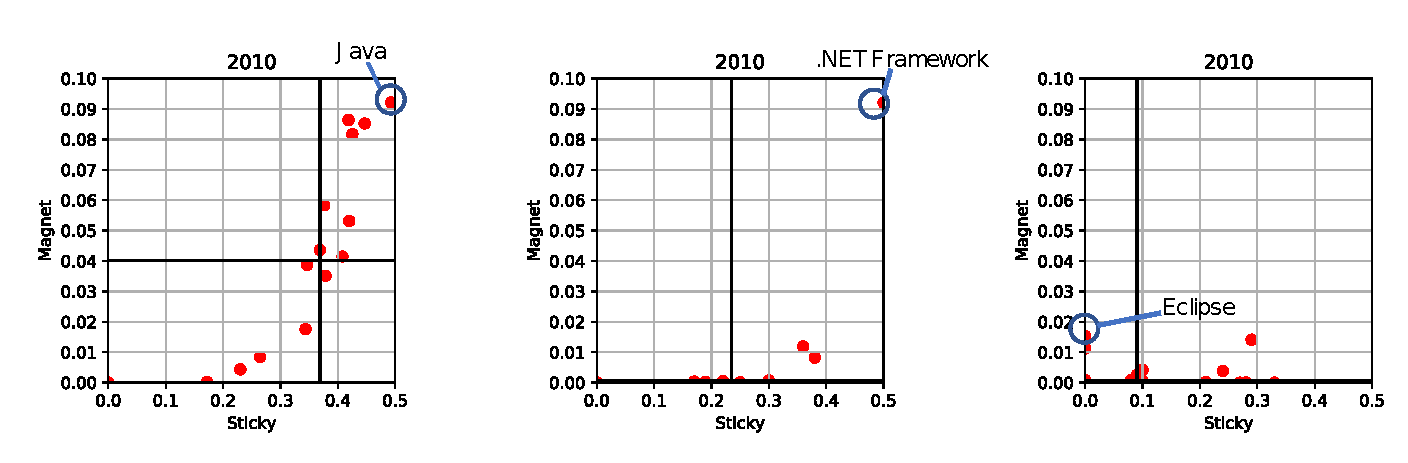
\includegraphics[width=1.0\hsize]{img/2010all.eps}  
 \caption{Distribution of Magnet and Sticky values in Prosgraming Language, Framework and Environment} 
 \label{fig:2010} 
\end{figure*}


\section{Dataset}
In this paper, we analyze the Stack Overflow dataset (SOTorrent) provided by Sebastian Baltes et al.~\cite{msr2019challenge}. SOTorrent is an open dataset based on the official SO data dump. SOTorrent provides access to the version history of SO content at the level of whole posts and individual text or code blocks.

The dataset includes 20 different tables which store not only data from official SO data dump but also data extracted from the original official SO data dump.

In this paper, we only analyze the data from table \emph{Posts} which includes about 42 million posts from Stack overflow and table \emph{Users} where there are about 9 million rows of user information from July 2008 to September 2018. We focus on  users, tags, and time information of questions.

In this paper, we consider a user to be one who asks or answers questions in Stack Overflow. Those who comment or like/unlike on questions or answers are not counted in the statistics.


\begin{table*}[t]
 \centering
 \caption{Quadrant Transition of Framework 2010 - 2018} 
 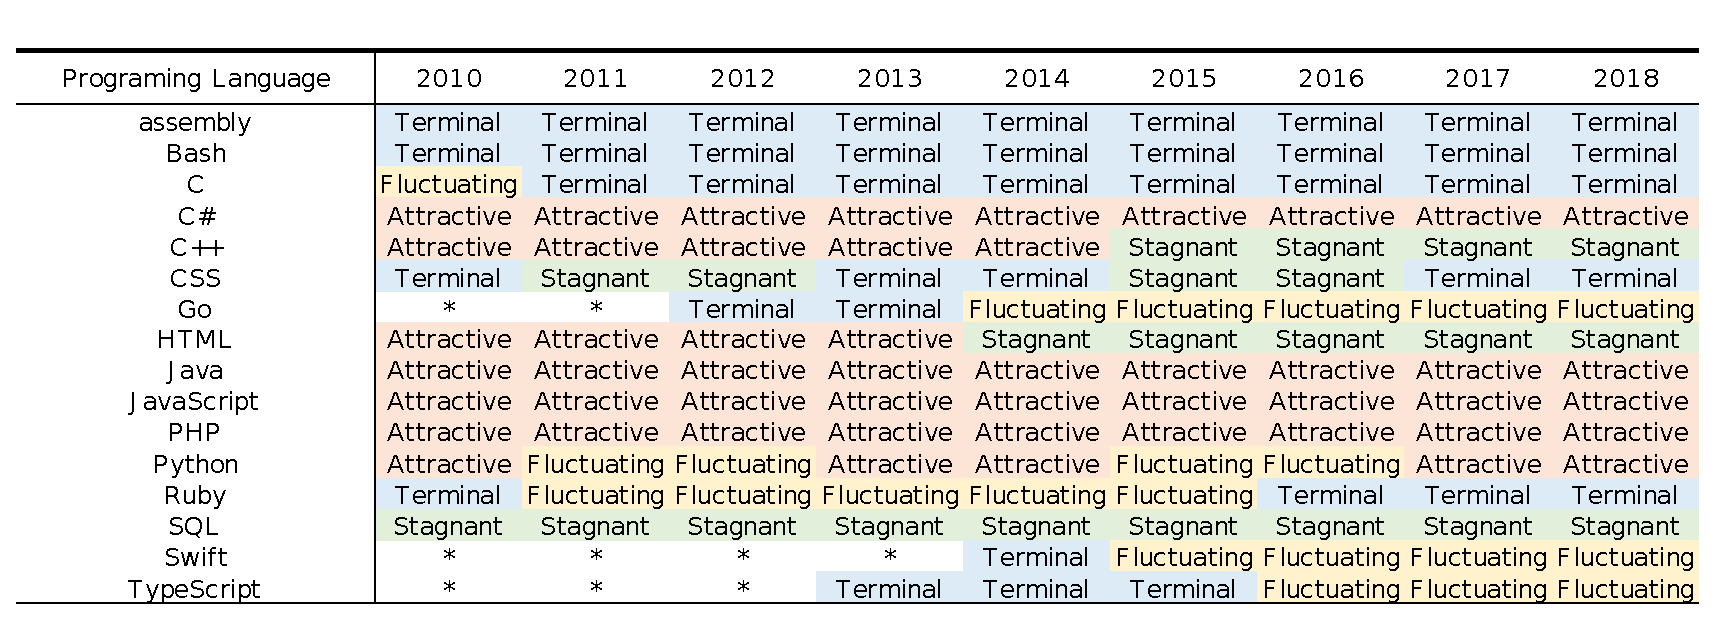
\includegraphics[width=1.0\hsize]{img/frame2010-2018.eps} 
 \label{table1} 
\end{table*}

\section{Study Results} %paragraph4
We set research results and faced two questions against these results. We discuss the questions based on the results.

\subsection{(RQ1) What are typical values of magnet and sticky in Stack Overflow?}

\noindent
\textbf{Approach.}
We have calculated magnet and sticky values as defined in Section \ref{magnet}. We plot the magnet value on the vertical axis and the sticky value on the horizontal axis. We classify the plotted points into 4 quadrants.\\
\textbf
{Attractive:} Tag with the high magnet and sticky value. By knowing attractive tags, we can find out what the developers are interested in.\\
\textbf{Fluctuating:} Tag with high magnet and low sticky value. This tag attracts people but it is short-term. Excellent developers will not continue to be interested.\\
\textbf{Stagnant:} Tag with the low magnet and high sticky value. These tags are difficult to attract new users but maintain existing users.\\
\textbf{Terminal:} Tag with the Low magnet and low sticky value. This tag can neither attract new users' developers nor keep them interested.

In this paper, the median of the magnet and sticky values for each year is used for the threshold of the quadrant because the median value is not much affected by outliers. As we showed the sticky value definition in Section \ref{magnet}, the sticky value depends on the number of tag users in that year and the following year. So in order to answer RQ1, we got 9 years' worth of sticky value from the information on the number of tag users from 2009 to 2018. The sticky value must depend on the number of new tag users but if the number of new tag users in the target year is too low, the sticky value will be too small. Therefore, in order to remove noise, we decided thresholds for each topic and when the magnet and sticky value is less than the threshold value, it is set to 0.


We did not analyze all the tags at once, but divided them into three categories for analysis. The categories we selected and their contents are:
\begin{itemize}
\item programming languages ​​(assembly, Bash, C, C♯, C ++, CSS, Go, HTML, Java, JavaScript, PHP, Python, Ruby, SQL, Swift, TypeScript)
\item frameworks ( .NET Framework, Angular, Cordova, Django, Hadoop, Node.js, React, Spark, Spring, TensorFlow, Torch, Xamarin)
\item environment (Android Studio, Atom Editor, Eclipse, Emacs, IntelliJ, IPython, Jupyter, NetBeans, Notepad++, PhpStorm, PyCharm, RStudio, RubyMine, Sublime Text, TextMate, Vim, Visual Studio, Visual Studio Code, Xcode)
\end{itemize}

We chose these tags based on Stack Overflow's survey of over 100,000 developers in 2018~\footnote{\url{https://insights.stackoverflow.com/survey/2018}}. We focused on tags used by more than 5\% of developers who answered the questionnaire. 

%The year when StackOverflow released these data is May 2008. Since the sticky value is calculated from the difference between the previous year and the current year, the distribution chart of magnet and sticky value according to three categories in 2010 is shown as the first year for which yearly data of sticky value can be obtained.

% 我々は全てのタグを一度に調査するのではなく3つのカテゴリに分けて分析をした。その方が特徴を見つけやすいからである。我々が選んだカテゴリたちとその内容はプログラミング言語(assembly, Bash, C, C♯, C++, CSS, Go, HTML, Java, JavaScript, PHP, Python, Ruby, SQL, Swift, TypeScript), フレームワーク(.NET Framework, Angular, Cordova, Django, Hadoop, Node.js, React, Spark, Spring, TensorFlow, Torch, Xamarin),そして環境(Android Studio, Atom Editor, Eclipse, Emacs, IntelliJ, IPython, Jupyter, NetBeans, Notepad++, PhpStorm, PyCharm, RStudio, RubyMine, Sublime Text, TextMate, Vim, Visual Studio, Visual Studio Code, Xcode)である。
% これらを選んだ理由は2018年にStack Overflowが10万人を超える開発者たちにとったアンケートの結果に基づいている。Stack Overflowは開発者たちに使用するタグたちについてのアンケートをとり、我々はアンケートに答えた開発者たちの5\%以上が使用しているタグたちに絞って調査した。StackOverflowがこれらのデータを公開した年は2008年5月である。sticky値は前年と当年の差から算出しているため、sticky valueの通年データが取れる最初の年として2010年の3カテゴリ別のmagnetとsticky valueの分布図を示す。

% The categories we selected and their contents are programming languages (assembly, Bash, C, C\#, C++, CSS, Go, HTML, Java, JavaScript, PHP, Python, Ruby, SQL, Swift, TypeScript), framework (.NET, Angular, Cordova, Django, Hadoop, Node.js, React, Spark, Spring, TensorFlow, Torch, Xamarin), and the environment (Android Studio, Atom Editor, Eclipse, Emacs, IntelliJ, IPython, Jupyter, NetBeans, Notepad++, PhpStorm, PyCharm, RStudio, RubyMine, Sublime Text, TextMate, Vim, Visual Studio, Visual Studio Code, Xcode) because these three categories are one of the most popular tag categories used in stack overflow. We also analyzed by picking the top tags that are popular among each category. Tags that are not popular have no character and we do not know anything from that. By dividing it for each category, it became easier to see the features. We show distribution map of magnet and sticky value by 3 categories of 2010 as one of the characteristics easy to understand.

%\textbf{Manual analysis:}
%Figure~\ref{fig:2010} shows the distribution of magnet and sticky values in programing language, framework, and environment (2010)\footnote{We choose the year 2010 because it is the first year for which yearly data of sticky value can be obtained.}. 
% We find that .NET Framework is a high magnet and sticky value. 

%.NET framework 

%Beginner developers can relatively easily develop advanced software using . Are there many reasons why the .NET Framework's sticky value is high reasons most conveniently? It is the foundation system for building applications. 

%Java has long been popular and attractive as it is one of the most famous programming languages ​​in the world. Eclipse especially attracted people in 2010, so the magnet value is high.

% 図~\ref{plotframe2010}の2009 Frameworkにおいて、.NET Frameworkは高いマグネットとスティッキー値である。高いマグネットとスティッキー値であることは非常に良いと言える。.NET Framework は、2006年11月にマイクロソフトに発表された。これはネットワーク上でアプリケーションを構築する基盤のシステムである。.NET Frameworkのmagnet valueが高い理由は、初心者エンジニアでもある程度高度なソフトウェアを開発できるからである。.NET Frameworkのsticky valueが高い理由はその利便性から長く使う人が多いからだ。
% 2009 Languageにおいて、C♯のmagnet valueとsticky valueは最も高い。これは.NET構想において、C♯が中心的な開発言語であり、そのフレームワークは.NET Frameworkであることが理由のように思われる。
% 2009 Environmentにおいて、Visual Studioが高いmagnet valueとsticky valueである。Visual Studioは.NET構想を作ったMicrosoftが作った最も代表的な開発環境である。PhpStormは高いsticky valueと低いmagnet valueである。PhpStormはPHPでの開発に向いており、それはコード補完の点で優れている。PHPで開発をしない人々にとってはあまり魅力的ではないが、PHPを使う人々にとっては非常に魅力的であるためこのような結果になったと思われる。
% \medskip

\noindent \textbf{Results:}
Figure~\ref{fig:2010} shows a quadrant plot of the magnet and sticky values ​​of the 2010 framework, programming language, environmental tag\footnote{We choose the year 2010 because it is the first year for which yearly data of sticky value can be obtained.}. We can see that the magnet value is lower than the value of sticky. This is similar findings with the investigation of the Pew Research Center. Like citizens are more likely to spend more time living on the same land than to change houses, it is easier for developers to continue developing about the same content.

 % \emph{Stickyの方がmagnetより一般的な属性である。高いmagnet valueのタグは初心者でも使いやすいものである。特に.NET Frameworkのようなmagnetなタグは比較的使いやすいものであるため初心者などに多く使われている。C♯のように古くからあり有名なタグはmagnet valueもsticky valueも高くAttractiveである。また.NETのように一つの優れた構想に関連のある環境やプログラミング言語もまた人気である。
  
\noindent
\textbf{Summary.}
 Tags with high magnet value are easy to use even for beginners. A tag that is familiar from old days like Java has a high magnet value and sticky value and is attractive.

\begin{table}[t]
 \centering
 \caption{Average Quadrant Transition rate}
 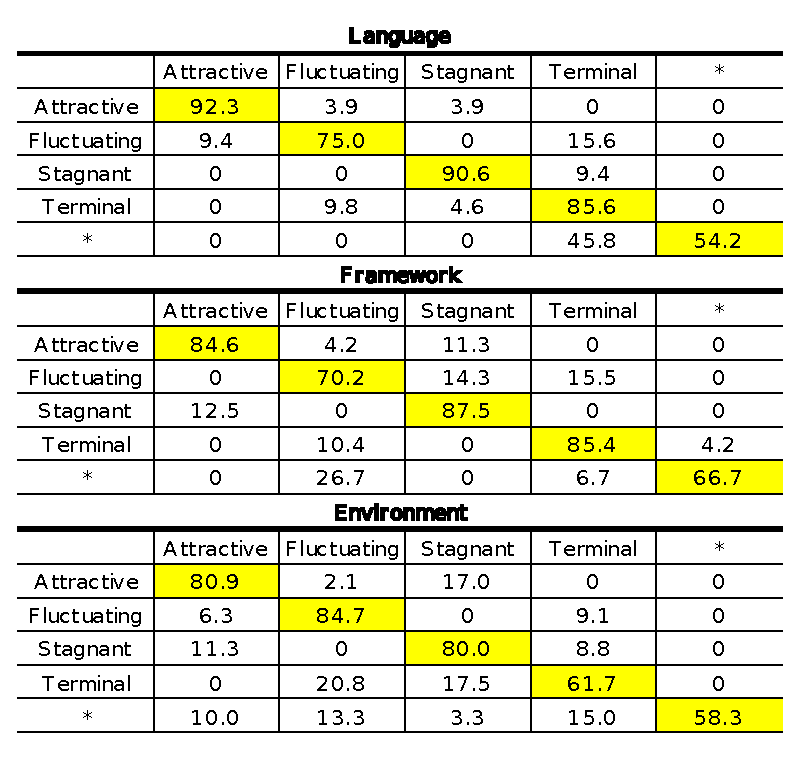
\includegraphics[width=1.0\hsize]{img/averageAFST.eps} 
 \label{table2} 
\end{table}

\subsection{(RQ2) How do magnet and sticky values change over time?} 

\noindent \textbf{Approach:}
From 2010 to 2018, we calculated the probability that the tags move quadrants from one year to the following year. For example, there are six Attractive tags in 2010. Of the six tags that were Attactive in 2010, there are five that were Attractive the following year as well. Therefore, the transition probability from Attractive to Attractive for 2010 - 2011 is 5/6 or 83.3\%. 

\noindent \textbf{Quantitative results:}
Table~\ref{table2} shows the proportion that the vertical axis is in that quadrant for some years up to 2010-2018, the horizontal axis is that year old. From the table, we can find that the ratio of tags that do not move the quadrants from the previous year to the following year is the highest in any field of programming language, framework, environment. Since the tags have hardly changed from any quadrant to *, once the tags have become popular to a certain extent, the users of the tags have not been significantly reduced since then. It also shows that once tags have become less popular, it will be difficult to become popular again.

\noindent \textbf{Manual analysis:}
Table~\ref{table1} shows the transition of each tag quadrant in the framework. From this table we can see how the tags move in the quadrant. Here we turn to Xamarin as an interesting example. Basically, Xamarin is an API for Android and iOS that can be called from C♯, so you can not develop an application without knowing both details. This means that if you start developing Android and iOS apps with Windows and Visual Studio you will need a lot of knowledge, which is not good for beginners. When Xamarin first appeared, it attracted attention as a tool that developers can efficiently develop. However, on sites where beginners often ask questions, such as StackOverflow, its popularity seems to have gradually declined due to its use difficulty.

About Riact, this is a JavaScript library from Facebook. It aims to build the user interface of web application efficiently. It was first used on Facebook's news feed in 2011 and in 2012 on Instagram. It was open sourced at JSConf US in May 2013. SNSs such as FaceBook and Instagram have begun to become popular around 2015-2016, when React has changed from Terminal to Floating. Therefore, it seems that the popularity of Framework that builds it to popular SNS has also changed.

% 表2はフレーフレームワークにおいて各タグの象限の変遷を示している。この表から、我々はタグたちがどのように象限を変遷していくかがわかる。ここで、面白い例としてXamarinに注目する。Xamarinは基本的にAndroid API,iOSのAPIをC♯から呼び出せるようにしたものなので、両者について知らないとアプリ開発ができない。つまりWindows と Visual StudioでAndroidとiOSアプリの開発を始める場合大変多くの知識を必要とするため初心者には向かない。Xamarinが登場した当初は開発者たちが効率よく開発できるツールとして注目を浴びたが、StackOverflowのように初心者が質問することが多いサイトにおいてはそのしよう難易度の高さから徐々に人気が減少していったのだろうと思われる。
% またRiactについて、これはFacebookとコミュニティによって開発されているユーザインタフェースを構築するためのJavaScriptライブラリである。2011年にFacebookのニュースフィード上で最初に使用され、2012年にはInstagramでも使用されるようになった。2013年5月のJSConf USでオープンソース化された。FaceBookやInstagramなどのSNSが人気になり始めたのはちょうどReactがTerminalからFluctuatingに変遷した2015-2016年ごろであるため、人気のSNSに合わせてそれを構築するFrameworkの人気も変化したのではないかと思われる。

% Table~\ref{table2} shows the transition of the quadrant of each tag in the framework. From this table we can see how the tags are turning quadrants.
% Table~\ref{table2} shows that framework tags often stay in the same quadrant. It turns out that tags frequently change between Attractive and Stagnant, Terminal and Fluctuating.
\smallskip\smallskip

\noindent \textbf{Summary:}
Even if it was a tool that was initially popular, its popularity would decline if it was difficult to use. Even if it was a tool that was not as popular as it was born, It turns out that as the content using the tool becomes popular, the tool also becomes popular

% \begin{oframed}
%\emph{Table~\ref{table1} shows that even if it was a tool that was initially popular, its popularity would decline if it was difficult to use. Even if it was a tool that was not as popular as it was born, It turns out that as the content using the tool becomes popular, the tool also becomes popular. Table~\ref{table2} shows that it is difficult for tags to make large changes in quadrants.}
% 表1から、タグたちは四分円を大きく変遷しづらいことがわかった。また表2から、たとえ当初人気があったツールだとしても、それが使いにくいあるいは使用するのが難しいものであればその人気は減少し、また誕生当初はそこまで人気がないツールだとしても、そのツールを使用しているコンテンツが人気になればそれに伴いそのツールも人気になることがわかった。

% As a result of investigating from 2009 to 2018, in the programming language, the average transition from Attractive to Attractive was 91.5\%, the transition from Fluctuating to Fluctuating was 77.8\%, the change from Stagnant to Stagnant was 80.6\%, and the change from Terminal to Terminal was 87.2\%.  Regardless of the kind of tag, it turned out that the classification of tags was difficult to change.
% \end{oframed}


\section{Conclusions}
Whether it is a programming language or a program framework or an operating system, keeping the community alive and attracting more people to participate in discussions is critical to its development. Especially on the stack overflow, the world's largest program Q\&A platform, having more questions and answers on a topic means that customers of the product are more likely to solve their own problems, which is even more tedious than that developers rack their brains to write a lengthy development document or Q\&A This paper applied the magnet and sticky population concepts to a set of topics in Stack Overflow. We find that:

1. The number of topics that people participate in is exploding with the development and popularity of computer technology. Even the most popular themes cannot attract the high percentage of people involved in the discussion like what they did ten years ago.
\smallskip\smallskip

2. Under their respective major categories, the most popular topics are still very popular after ten years, and only a small number of languages or frameworks can stand out and become one of the most popular topics.
\smallskip\smallskip

3. This research can provide some reference for enterprises to choose their own main technology stack, and can also be used as a reference for computer science students to learn new technologies, because it (1) predicts the trend of computer technology in the next few years, (2) points out which technologies are easier to access and the questions can be easier to get answers to.

\bibliographystyle{IEEEtran}
\bibliography{mining}

\end{document}
